\chapter{Inferenza di Alberi Tumorali tramite Particle Swarm Optimization}
\label{chap:pso}
In questa sezione verrà descritto lo strumento di inferenza di alberi tumorali tramite Particle Swarm Optimization (d'ora in poi \textbf{PSO}), le ipotesi effettuate, i risultati ottenuti ed eventuali conclusioni. Viene utilizzata la tecnica euristica Particle Swarm Optimization, descritta precedentemente nel \autoref{chap:intro-optim-pso}.

\section{Strumenti Utilizzati}
Lo strumento è stato sviluppato in Python. Inizialmente si era cercato di utilizzare Cython\footnote{Un linguaggio di programmazione simile a Python, ma con il vantaggio di avere velocità simili a quelle ottenute da C}, poi abbandonato poiché lo studio di questo linguaggio di programmazione avrebbe ridotto il tempo utile alla vera e propria implementazione dello strumento. Si pensa però in futuro di riscrivere il codice utilizzando \textit{C++}.

L'ambiente di sviluppo scelto è \textit{Visual Studio Code}, con l'ausilio delle estensioni di debugging per Python. In generale sono sempre stati utilizzati strumenti che seguono la filosofia \textit{Open Source}, di conseguenza questa tesi ed il codice sviluppato saranno entrambi disponibili liberamente sul profilo GitHub \cite{mygithub} del sottoscritto sotto licenza GPL3 e MIT rispettivamente.

I moduli e le librerie Python che sono state utilizzate sono elencate di seguito: \begin{itemize}
  \item \pyref{random} -- modulo standard che implementa funzioni per la generazione di numeri pseudo-randomici
  \item \pyref{multiprocessing} -- modulo standard utilizzato per implementare il supporto di parallelizzazione e gestione della concorrenza
  \item \pyref{sys} -- modulo standard per accedere ad alcune variabili o funzioni di sistema
  \item \pyref{time} -- modulo standard usato per accedere a funzioni relative al tempo, come l'accesso all'ora attuale, o per la misurazione dei tempi di esecuzione
  \item \pyref{math} -- modulo standard che permette l'accesso a funzioni ottimizzate per il calcolo matematico
  \item \pyref{copy} -- modulo standard utilizzato per copiare in profondità degli oggetti, con un nuovo puntatore all'oggetto
  \item * \pypi{graphviz} -- modulo esterno per la visualizzazione ed il salvataggio su file dei grafi da formato graphviz\footnote{Strumento che permette di disegnare rappresentare dei grafi utilizzando la notazione DOT, un linguaggio che descrive la struttura di grafi generici}
  \item * \pypi{ete3} -- modulo esterno utilizzato come base di appoggio per le funzioni essenziali relative ai nodi di un albero, come la ricerca dei nodi e l'aggiunta o rimozione di essi
  \item * \pypi{networkx} -- modulo esterno sfruttato per il calcolo del \textit{maximum weight matching}
\end{itemize}

\small * Moduli esterni

\subsection{Dati utilizzati}
Per poter testare l'algoritmo ed il codice sviluppato su di esso è essenziale avere dei dati sia veri che simulati. A questo proposito sono stati utilizzati i dati simulati dal laboratorio di appartenenza del progetto, AlgoLab. Nelle seguenti sezioni verranno analizzati i dati relativi al file simulato presente nella directory del progetto \texttt{data/simulatex/exp1/sim1\_scs.txt}.
% TODO: spiegare perché è utile avere sia dati veri che simulati

\section{Adattamento del problema a Particle Swarm Optimization}
\label{chap:pso-adapt}
Una delle principali sfide in questo progetto è stata di riuscire a trovare un'interpretazione valida ed efficacie adatta alla tecnica euristica scelta, appunto il Particle Swarm Optimization, il cui funzionamento ed algoritmo sono descritti dettagliatamente nella \autoref{chap:intro-optim-pso}. Il modello più immediato da adattare al problema è quello di associare una particella dello swarm ad un albero sul quale vengono effettuate delle operazioni. Queste operazioni saranno ciò che determina il ``movimento'' della particella nello spazio. Lo swarm non è quindi altro che l'insieme degli alberi. Possiamo dividere l'implementazione in quattro fasi: \begin{enumerate}
  \item Inizializzazione
  \item Calcolo del movimento della particella
  \item Aggiornamento della particella
  \item Aggiornamento della particella migliore dello swarm e della soluzione migliore della particella
\end{enumerate}

\section{Modello degli errori single-cell}
\label{chap:pso-matrix}
I dati single-cell vengono rappresentati tramite un modello di sostituzione come quello illustrato nella \autoref{chap:intro-models} tramite una matrice $M = n \times m$, con $n$ cellule e $m$ mutazioni. Viene poi utilizzata una matrice $D = n \times m$ è ricavata dall'osservazione dell'albero inferito, ed è una versione imperfetta del vero genotipo della matrice $M$. Per mitigare i problemi causati dalle tecniche di WGA (\autoref{chap:intro-scs}) viene utilizzato il parametro $\alpha$ per indicare la probabilità di incontrare un falso positivo, quindi osservare un $1$ quando in realtà questo è uno $0$, e falsi negativi, cioè di avere la probabilità $\beta$ di osservare uno $0$ quando in realtà è un $1$:
\begin{align}
    \label{eq:pso-intro-model-matrix}
    \begin{split}
      P(M_{i,j} = 0 | D_{i,j} = 0) = 1 - \alpha, \qquad
      &P(M_{i,j} = 0 | D_{i,j} = 1) = \beta, \\
      P(M_{i,j} = 1 | D_{i,j} = 0) = \alpha, \qquad
      &P(M_{i,j} = 1 | D_{i,j} = 1) = 1 - \beta
    \end{split}
\end{align}

\subsection{Inizializzazione}
\label{chap:pso-adapt-init}
Possiamo considerare una particella dello swarm come un albero, la cui posizione è determinata dalla configurazione dei suoi nodi. L'inizializzazione viene effettuata randomizzando la topologia di un albero binario $T$ con $m$ nodi, uno per ogni mutazione, con una funzione randomica\footnote{In realtà la funzione è del tipo pseudo-randomica, utilizzando il generatore \textit{Mersenne Twister} \cite{Matsumoto:MersenneTwister}, ma non avendo problemi dal punto di vista della sicurezza o della riproducibilità, è stato pervenuto che per i nostri scopi è più che valido e sufficiente}. In questo modo, viene ottenuta una topologia simile a quella rappresentata nella \autoref{fig:pso-adapt-init-topology}. Il metodo di generazione dell'albero binario è ripreso da quello implementato su SASC, ed è descritto nell'\autoref{algo:pso-adapt-init}.

\begin{algorithm}[!h]
    $m = $ numero di mutazioni
    $r = $ radice dell'albero \\
    $tree = [1, \dots, m]$ \Comment{Vettore con tutti i nodi dell'albero}
    random.shuffle(tree) \Comment{Il vettore dei nodi viene randomizzato}
    $nodes \gets [r]$ \\
    $append\_node \gets 0$ \\
    \While{$i < m$}{
      newNode $\gets$ new Node(name $=$ mutation\_name(m), parent $=$ nodes[append\_node], mutationid $=$ tree[i]) \\
      nodes.append(newNode) \\
      $i \gets i + 1$ \\
      \If{$i < m$}{
        newNode $\gets$ new Node(name = mutation\_name(m), parent = nodes[append\_node], mutationid = tree[i]) \\
        nodes.append(newNode)
      }
      append\_node $\gets$ append\_node $+ 1$
      $i \gets i + 1$
    }
    \Return{r}
    \caption{RandomTreeInit}
    \label{algo:pso-adapt-init}
\end{algorithm}

\begin{figure}[!h]
  \centering
  \begin{forest}
      germline
      [{germline}
      [{6} 
      [{18} 
      [{28} 
      [{11}  ]
      [{8}  ] ]
      [{24} 
      [{21}  ]
      [{14}  ] ] ]
      [{10} 
      [{30} 
      [{9}  ]
      [{17}  ] ]
      [{29} 
      [{1}  ]
      [{3}  ] ] ] ]
      [{23} 
      [{27} 
      [{20} 
      [{19}  ]
      [{16}  ] ]
      [{15} 
      [{12}  ]
      [{13}  ] ] ]
      [{2} 
      [{26} 
      [{7}  ]
      [{22}  ] ]
      [{4} 
      [{25}  ]
      [{5}  ] ] ] ]]
    \end{forest}    
  \caption{Esempio di topologia iniziale con $m = 30$}
  \label{fig:pso-adapt-init-topology}
\end{figure}

La complessità di questo algoritmo è facilmente espressa da $O(m)$, poiché viene creato un nodo per ogni mutazione.

\subsection{Calcolo del movimento di una particella}
\label{chap:pso-adapt-calculate}
La seconda fase è il calcolo della velocità con la quale una particella si muove rispetto a $p_i$ e $g$, cioè l'albero migliore che ha avuto la particella fino ad ora, e l'albero migliore in tutto lo swarm. Come parametro di paragone è definita la likelihood logaritmica descritta nell'\autoref{eq:art-sasc-lh}.

Questo step è stato uno dei problemi principali da affrontare sin dal principio del progetto. Non è immediato trovare un modello diretto che rappresenti la velocità e la direzione di una particella verso gli alberi migliori $p_i$ e $g$, data la natura non lineare del problema. Sono state, dunque, introdotte diverse metriche (o assenza di tali) per cercare di definire al meglio questo parametro in maniera tale che aderisse al meglio all'algoritmo scelto, quindi PSO. Nelle seguenti sottosezioni verranno descritti tali esperimenti, con risultati e considerazioni del caso.

La complessità della solo ricerca di un modello per il parametro della velocità ha portato a tralasciare, almeno temporaneamente, altri fattori presenti nel PSO originale, quali ad esempio l'\textit{attrito} ($\omega$) ed i \textit{learning factors} ($\phi_p, \phi_g$), fattori moltiplicativi utili per velocizzare o rallentare il comportamento di scalata della collina dell'algoritmo.

\subsubsection{Assenza del parametro di velocità}
\label{chap:pso-adapt-calculate-1}
Nei momenti iniziali di questo progetto, come è stato descritto precedentemente, trovare una corrispondenza congeniale ed adeguata all'idea di \textit{velocità} del PSO è stato impegnativo. Al fine comunque di poter dare un via al lavoro, una delle prime metriche adottate di velocità è stata la vera e propria assenza di tale metrica. I risultati descritti nella \autoref{fig:pso-adapt-calculate-1-table} possono sembrare promettenti, dato che comunque provano la funzionalità del programma, e che la likelihood aumenta. Quello che i dati non ci dicono è però qualcosa che possiamo intuire dall'intrinseco comportamento dell'assenza della velocità come metrica: siamo di fronte ad un semplice algoritmo di highest hill climbing, descritto nella \autoref{chap:intro-optim-hill}. Quello che succede quindi è che si cerca di migliorare l'algoritmo al primo miglioramento individuato, in questo caso corrisponde ad ogni volta che si trova una likelihood migliore. Questo può sembrare un ottimo risultato, ma è in realtà un problema. L'estrema e ripida scalata rischia di incastrare la ricerca in un ottimo locale, peggiorando considerevolmente le possibilità di trovare un albero filogenetico di \textbf{buona qualità}. È importante sottolineare la \textit{bontà} del risultato, e non il basso valore della \textit{likelihood}, in quanto questo è solo un valore indicativo della verosomiglianza dell'albero con i dati a nostra disposizione, ma non dell'effettiva qualità della loro rappresentazione. È molto meglio quindi cercare di trovare un albero filogenetico con una qualità migliore che quello con la likelihood più elevata.

L'algoritmo risultante per il calcolo della posizione della particella risulta quindi essere il seguente:

\begin{algorithm}[!h]
    $r \gets random()$ \\
    \If{$r < .33$}{
      $tree \gets p_i$
    }
    \ElseIf{$r < .66$}{
      $tree \gets g$
    }
    \Else{
      $tree \gets x_i$
    }
    $execute\_random\_operation(tree)$
    \caption{ParticleIteration}
    \label{algo:pso-adapt-calculate-1}
\end{algorithm}
\begin{table}[!h]
  \centering
  \begin{tabular}{*{5}{c}}
    Particelle & Iterazioni & Likelihood Iniziale & Likelihood Migliore & CPU Time (s) \\ \midrule \midrule
    5 & 20 & -8865.28530 & -5807.87168 & 8.622138 \\
    10 & 20 & -8865.28530 & -3096.03633 & 17.478406 \\
    50 & 20 & -8341.99269 & -2258.47350 & 88.392956 \\
    85 & 20 & -8341.99269 & -1681.11579 & 153.431512 \\
    100 & 20 & -8341.99269 & -1650.24923 & 193.255694 \\
    150 & 20 & -8163.91004 & -1199.30190 & 275.721155 \\
    200 & 20 & -7944.95031 & -1173.53898 & 370.858453
  \end{tabular}
  \caption{Risultati ottenuti con assenza della velocità usando i parametri: $\alpha = 0.25, \beta = 1*10^{-5}, k = 3, seed = 1, n = 150, m = 30$}
  \label{tab:pso-adapt-calculate-1-table}
\end{table}
\begin{figure}[!h]
  \centering
  \begin{minipage}{.45 \textwidth}
  \centering
  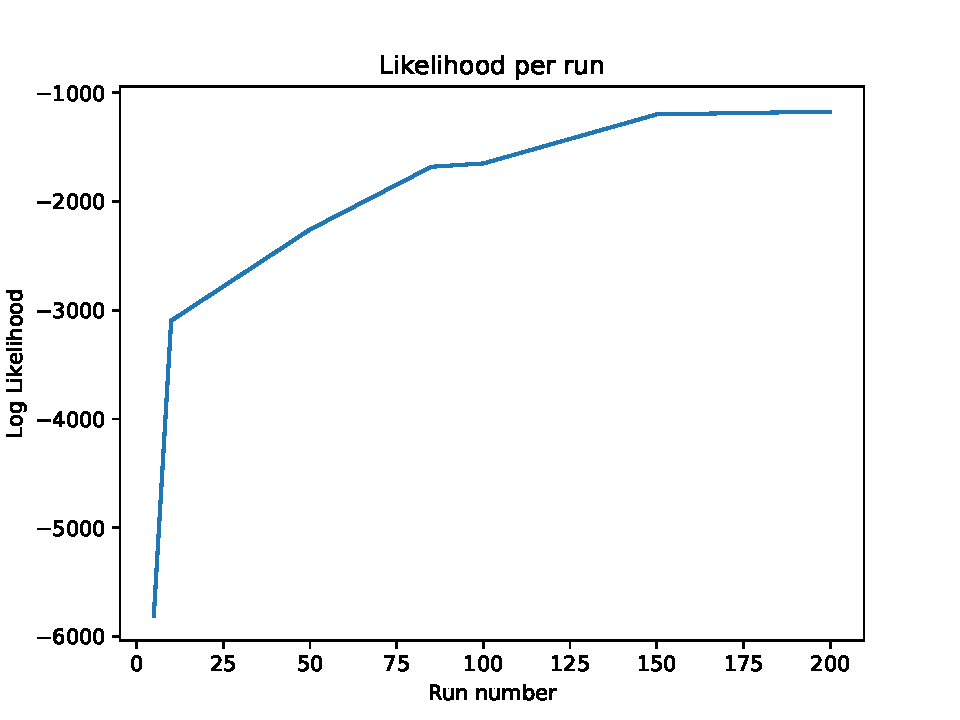
\includegraphics[width=0.8 \textwidth]{3221_lh.pdf}
  \caption{Grafico della likelihood sui vari parametri delle particelle con l'assenza della velocità}
  \end{minipage}
  \begin{minipage}{.45 \textwidth}
    \centering
    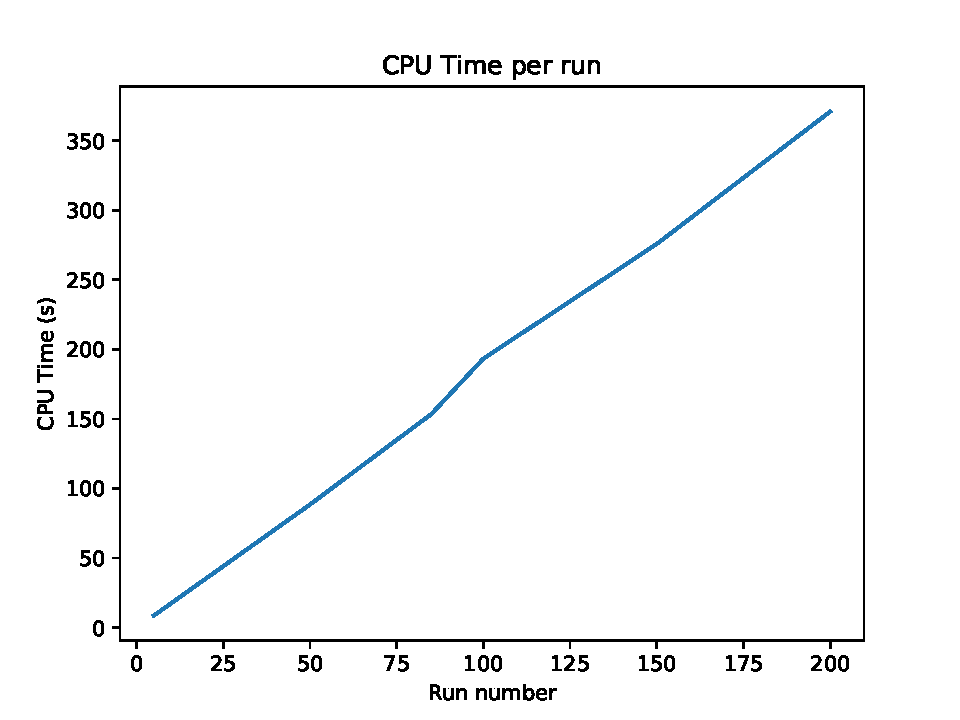
\includegraphics[width=0.8 \textwidth]{3221_cpu.pdf}
    \caption{Grafico del tempo sui vari parametri delle particelle con l'assenza della velocità}
  \end{minipage}
  \label{fig:pso-adapt-calculate-1-graph}
\end{figure}
\begin{figure}[!h]
  \centering
  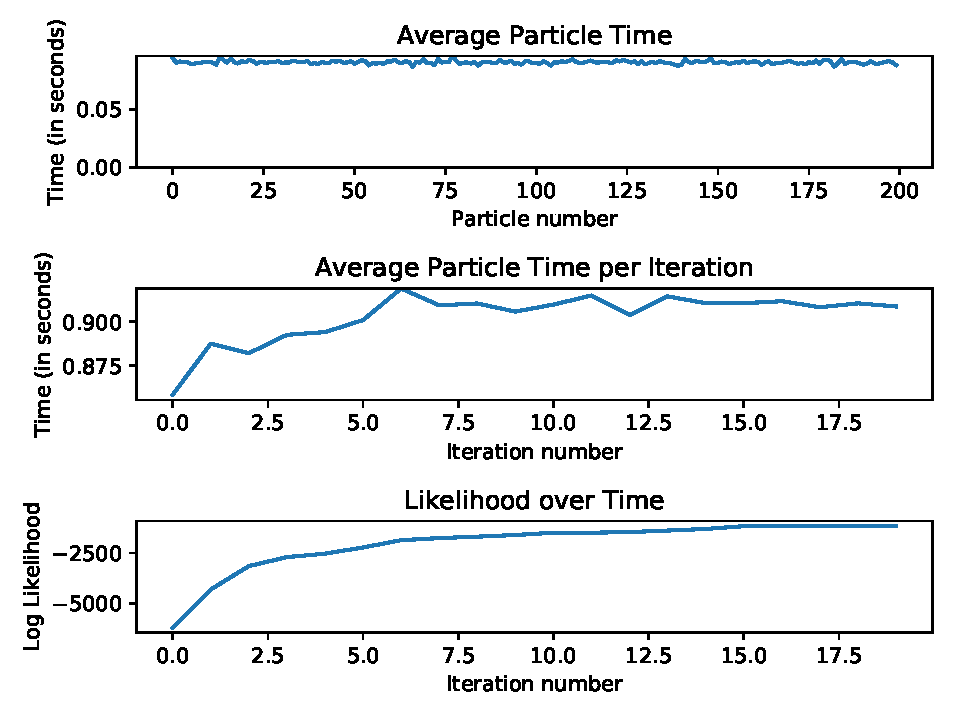
\includegraphics[width=0.8 \textwidth]{3221_data.pdf}
  \caption{Grafici sui tempi ed il miglioramento della likelihood con l'assenza della velocità}
  \label{fig:pso-adapt-calculate-4-data}
\end{figure}
\begin{figure}[!h]
  \centering
  \scalebox{0.7}{
  \begin{forest}
    germline
    [{germline} 
    [{29} 
    [{21} 
    [{22} 
    [{20} 
    [{4} 
    [{13} 
    [{1} 
    [{3} 
    [{19} 
    [{30} 
    [{25} 
    [{18} 
    [{23} 
    [{28} 
    [{11} 
    [{27} 
    [{17} ]]
    [{16} 
    [{12} 
    [{5} 
    [{9} 
    [{26} ]
    [{6} ]]]
    [{8} 
    [{7} ]]]]
    [{28},color=red 
    [{10} ]]
    [{15} ]]]]]
    [{3},color=red 
    [{30},color=red ]]]]]]
    [{24} ]
    [{14} 
    [{2} ]]]]]]]]]]
  \end{forest}
  }
  \caption{Albero inferito con il metodo nella \autoref{chap:pso-adapt-calculate-1}, $likelihood = -1173.53898$}
  \label{fig:pso-adapt-calculate-1-tree}
\end{figure}

\subsubsection{Prima metrica per la distanza tra filogenie}
\label{chap:pso-adapt-calculate-2}
Non avere un parametro della velocità è quindi un problema abbastanza importante, e preclude il poter continuare a sviluppare il progetto sotto le condizioni dello sviluppo di un algoritmo genetico di tipo PSO.
Ci si è quindi concentrati sullo studio di una metrica che permetta di trovare la distanza tra due alberi filogenetici. Il risultato di tale lavoro è stata la formulazione dell'\autoref{eq:pso-adapt-calculate-2-algo-1}. Per il \textit{max\_weight\_matching} (descritto nella \autoref{chap:intro-extra-matching-maxw}) si assume che il grafo $G = (V, E)$ sia formato da tutti i nodi del primo albero, $T_1$ e del secondo albero, $T_2$, in maniera tale da creare un \textit{grafo bipartito}\footnote{Un grafo bipartito è un grafo tale che l'insieme dei suoi vertici si può partizionare in due sottoinsiemi tali che ogni vertice di una di queste due parti è collegate solo a vertici dell'altra}, e la funzione peso $w: E \rightarrow \mathbb{N}$ indica il numero di mutazioni comuni tra due clade (\autoref{chap:intro-clade}). Il max weight matching restituisce un arco il cui peso è il massimo rispetto a quello di tutti gli altri archi presenti nel grafo bipartito. Il risultato della formula dovrebbe risultare $0$ quando $T_1, T_2$ rappresentano lo stesso albero, mentre $> 0$ quando differiscono.

\begin{equation}
  \label{eq:pso-adapt-calculate-2-algo-1}
  dist(T_1, T_2) = mutations - max\_weight\_matching(T_1, T_2)
\end{equation}

Un'analisi più approfondita della formula fa però emergere  un problema. La somma delle mutazioni comuni calcolata dalla funzione $w$ cresce all'aumentare della profondita in cui si trova il nodo nell'albero, poiché acquisisce più mutazioni. Un esempio è rappresentato nella \autoref{fig:pso-adapt-calculate-2-msum}.

\begin{figure}[!h]
  \centering
  \begin{minipage}{.45 \textwidth}
  \centering
  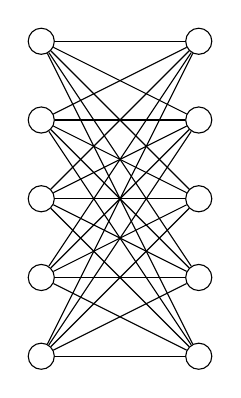
\begin{tikzpicture}[every node/.style={circle, draw}]
    \node at (0, 1) (a1) {};
    \node at (0, 2) (a2) {};
    \node at (0, 3) (a3) {};
    \node at (0, 4) (a4) {};
    \node at (0, 5) (a5) {};

    \node at (2, 1) (b1) {};
    \node at (2, 2) (b2) {};
    \node at (2, 3) (b3) {};
    \node at (2, 4) (b4) {};
    \node at (2, 5) (b5) {};

    \draw(a1) -- (b1);
    \draw(a1) -- (b2);
    \draw(a1) -- (b3);
    \draw(a1) -- (b4);
    \draw(a1) -- (b5);

    \draw(a2) -- (b1);
    \draw(a2) -- (b2);
    \draw(a2) -- (b3);
    \draw(a2) -- (b4);
    \draw(a2) -- (b5);

    \draw(a3) -- (b1);
    \draw(a3) -- (b2);
    \draw(a3) -- (b3);
    \draw(a3) -- (b4);
    \draw(a3) -- (b5);

    \draw(a4) -- (b1);
    \draw(a4) -- (b2);
    \draw(a4) -- (b3);
    \draw(a4) -- (b4);
    \draw(a4) -- (b5);

    \draw(a5) -- (b1);
    \draw(a5) -- (b2);
    \draw(a5) -- (b3);
    \draw(a5) -- (b4);
    \draw(a5) -- (b5);


  \end{tikzpicture}
  \caption{Esempio di grafo bipartito}
  \label{fig:pso-adapt-calculate-2-bip}
  \end{minipage}
  \begin{minipage}{.45 \textwidth}
    \centering
    \begin{forest}
      germline
      [{germline} 
      [{a} 
      [{b} 
      [{c} 
      [{d} ]]]]]
    \end{forest}\caption{Somma delle mutazioni acquisite per $max(d) = 4$}
    \begin{forest}
      germline
      [{germline}
      [{a}
      [{b} ]
      [{c}
      [{d} ]]]]
    \end{forest}
    \caption{Somma delle mutazioni acquisite per $max(d) = 3$}
    \label{fig:pso-adapt-calculate-2-msum}
  \end{minipage}
\end{figure}

Questo risulta in un calcolo della distanza che può risultare negativo, ed è quindi stato necessario adattare la metrica.

\subsubsection{Seconda metrica per la distanza tra filogenie}
\label{chap:pso-adapt-calculate-3}
L'analisi effettuata precedentemente ha portato alla formulazione di una nuova metrica (\autoref{eq:pso-adapt-calculate-2-algo-1}), stavolta rivelatasi corretta. D'ora in avanti verrà utilizzata questa metrica per la distanza tra due filogenie.

\begin{equation}
  \label{eq:pso-adapt-calculate-2-algo-1}
  dist(T_1, T_2) = max \{ \sum_{x \in T_1} m(x), \sum_{x \in T2} m(x) \} - max\_weight\_matching(T_1, T_2)
\end{equation}

L'algoritmo utilizzato per il maximum weight matching è quello presente all'interno della libreria \pypi{networkx}, 
richiamabile con \texttt{networkx.algorithms.matching.max\_weight\_matching(G)}, ed ha come complessità generale $O(n^3)$. A questo si vanno a sommare i tempi per il calcolo delle mutazioni in comune, che risulta essere $O(n^2 + nm)$ ed il calcolo del numero di mutazioni di un albero $O(n \cdot m)$. In totale, la complessità dell'algoritmo per il calcolo della distanza risulta essere $O(n^3 + n^2 + nm)$.

\subsubsection{Hill climbing con considerazione della distanza}
\label{chap:pso-adapt-calculate-4}
Ora che è stata definita una metrica per la distanza, è possibile iniziare a ragionare in maniera più analoga sulla velocità rispetto a quanto non si faceva prima. Si è pensato quindi di utilizzare la nuova metrica introdotta per calcolare la distanza tra la particella attuale $x_i$ e le due particelle migliori $p_i$ e $g$, e scegliere il clade con meno mutazioni in comune tra l'albero meno distante tra i due. Il clade scelto randomicamente viene poi inserito randomicamente come figlio di un nodo dell'albero attuale, e le mutazioni duplicate rimosse. Nella teoria questo avrebbe dovuto portare ad un graduale avvicinamento della particella attuale verso l'ottimo, nella pratica l'implementazione seguita è risultata, ancora una volta, in un algoritmo di hill climbing.
Eseguendo gli stessi test effettuati nella \autoref{chap:pso-adapt-calculate-1} si ottengono i risultati rappresentati nella \autoref{fig:pso-adapt-calculate-4-table}. 

\begin{table}[!h]
  \centering
  \begin{tabular}{*{5}{c}}
    Particelle & Iterazioni & Likelihood Iniziale & Likelihood Migliore & CPU Time (s) \\ \midrule \midrule
    5 & 20 & -8865.28530 & -7267.75496 & 19.66558 \\
    10 & 20 & -8865.28530 & -3207.95706 & 43.66173 \\
    50 & 20 & -8341.99268 & -2773.96311 & 239.89298 \\
    85 & 20 & -8341.99268 & -1664.407183 & 430.08543 \\
    100 & 20 & -8341.99268 & -1720.876536 & 602.24159 \\
    150 & 20 & -8163.91004 & -1594.589690 & 825.43232 \\
    200 & 20 & -7944.95031 & -1360.172665 & 1147.3371 \\
  \end{tabular}
  \caption{Risultati ottenuti con considerazione della distanza usando i parametri: $\alpha = 0.25, \beta = 1\cdot 10^{-5}, k = 3, seed = 1, n = 150, m = 30$}
  \label{tab:pso-adapt-calculate-4-table}
\end{table}

Si può evidenziare dal test effettuato come i tempi siano quasi duplicati, quasi triplicati, relativamente al fatto che vengono effettuati dei test sulla distanza che incidono negativamente sulle prestazioni. È però da notare che questo aumento dei tempi non coincide con un miglioramento sostanziale della ricerca dell'ottimo da parte dell'algoritmo, ma anzi, sia in media peggiorata. Questo può essere causa di vari fattori, tra cui la possibilità che l'algoritmo si comporti allo stesso modo di quello presentato nella \autoref{chap:pso-adapt-calculate-1}, ma l'introduzione di un nuovo passaggio dell'hill climbing abbia rallentato e peggiorato la scalata. Un esempio dell'albero inferito con 200 particelle è rappresentato nella \autoref{fig:pso-adapt-calculate-4-tree}, mentre i dati relativi all'andamento del tempo di calcolo e della likelihood nel corso delle varie iterazioni sono rappresentati in \autoref{fig:pso-adapt-calculate-4-data}.

\begin{figure}[!h]
  \centering
  \begin{minipage}{.45 \textwidth}
  \centering
  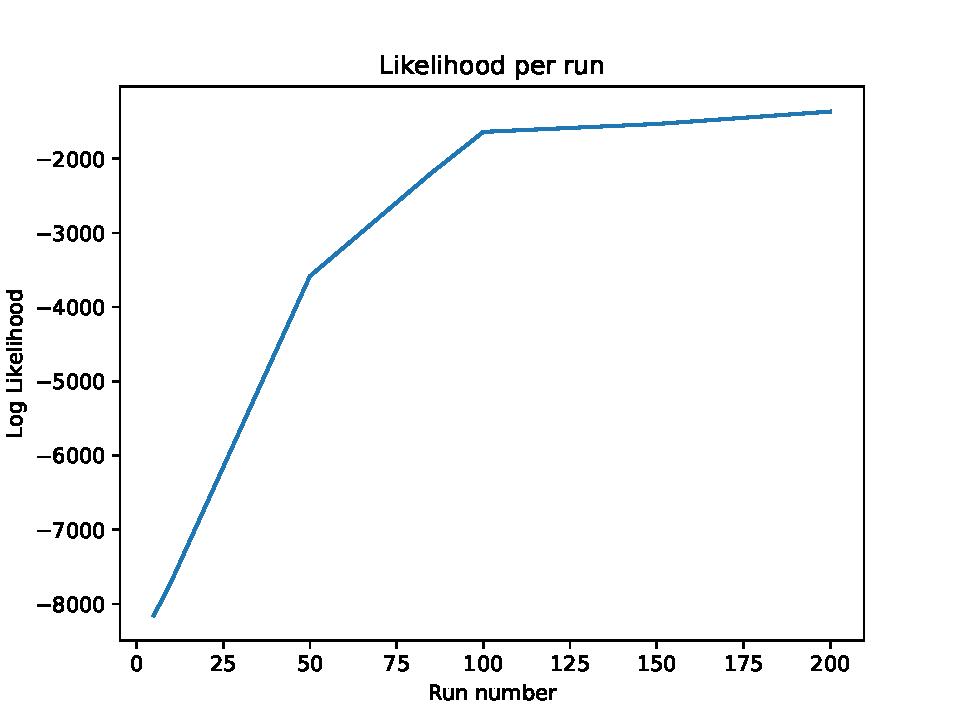
\includegraphics[width=0.8 \textwidth]{3224_lh.pdf}
  \caption{Grafico della likelihood sui vari parametri delle particelle con considerazione della distanza}
  \end{minipage}
  \begin{minipage}{.45 \textwidth}
    \centering
    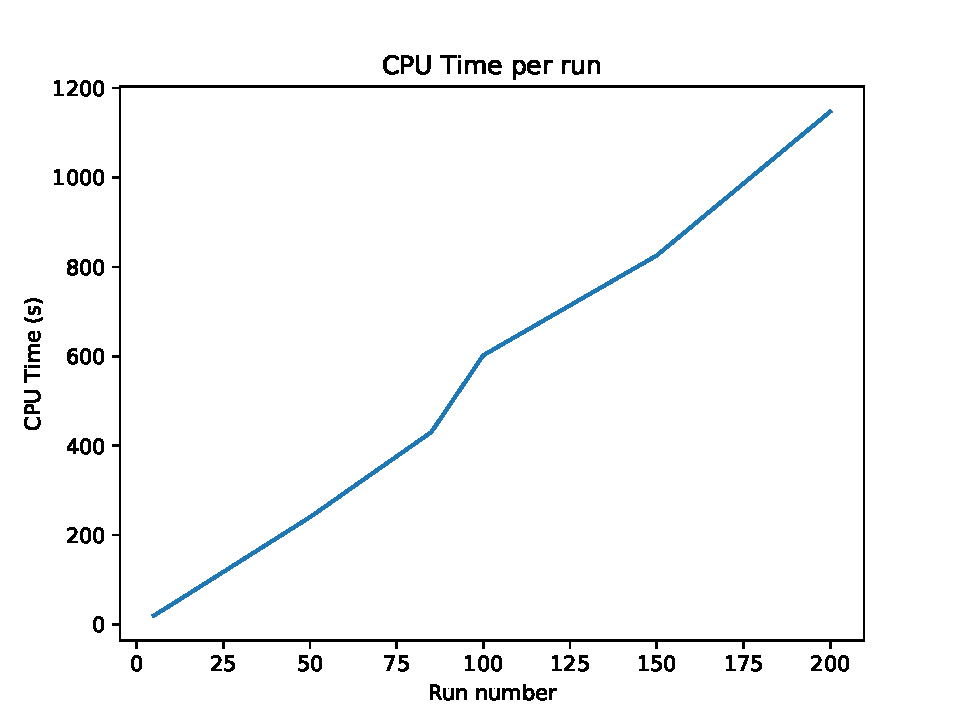
\includegraphics[width=0.8 \textwidth]{3224_cpu.pdf}
    \caption{Grafico del tempo sui vari parametri delle particelle con considerazione della distanza}
  \end{minipage}
  \label{fig:pso-adapt-calculate-1-graph}
\end{figure}

\begin{figure}[!h]
  \centering
  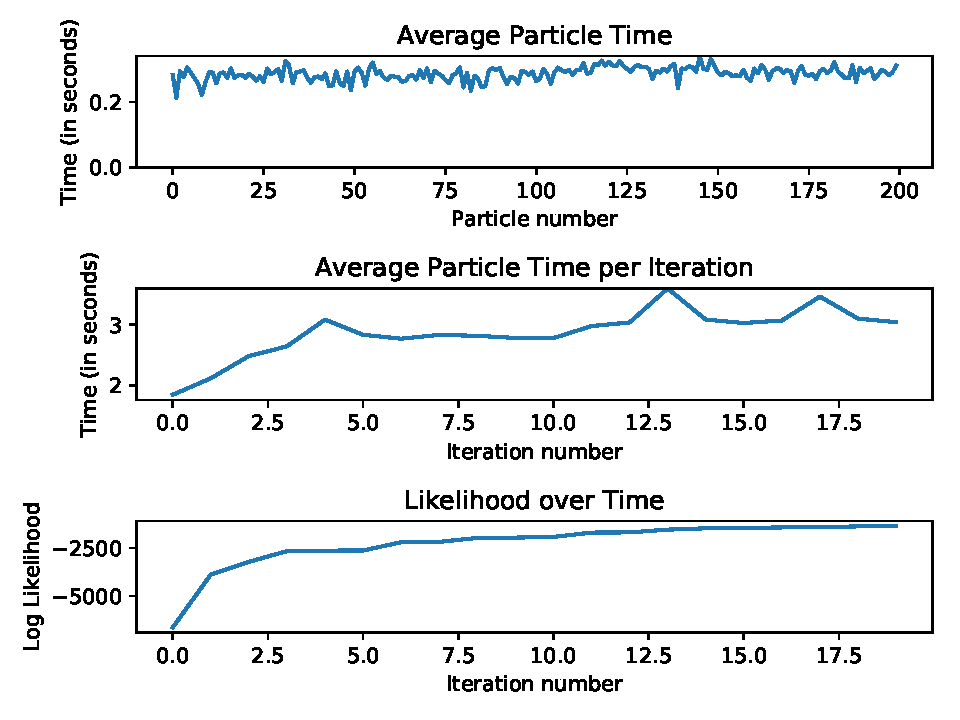
\includegraphics[width=0.8 \textwidth]{3224_data.pdf}
  \caption{Grafici sui tempi ed il miglioramento della likelihood con il passare del tempo}
  \label{fig:pso-adapt-calculate-4-data}
\end{figure}

\begin{figure}[!h]
  \centering
  \scalebox{0.7}{
    \begin{forest}
      germline
      [{germline} 
      [{20} 
      [{13} 
      [{1} 
      [{11} 
      [{21} 
      [{25} 
      [{22} 
      [{29} 
      [{18} 
      [{30} 
      [{19} 
      [{3} 
      [{4} 
      [{28} 
      [{10} 
      [{17} ]]
      [{27} ]]
      [{8} ]
      [{29},color=red 
      [{4},color=red ]]]
      [{16} ]]]
      [{25},color=red 
      [{23} 
      [{2} 
      [{14} ]]
      [{26} ]
      [{6} 
      [{9} 
      [{12} ]
      [{5} ]]]]]
      [{7} ]]]]]]
      [{24} ]]]]]
      [{15} ]]]
    \end{forest}
  }
  \caption{Albero inferito con il metodo nella \autoref{chap:pso-adapt-calculate-4}, $likelihood = -1540.622970$}
  \label{fig:pso-adapt-calculate-4-tree}
\end{figure}
\subsubsection{Clade casuali tra $p_i$ e $g$ come avvicinamento all'ottimo}
\label{chap:pso-adapt-calculate-5}
Fin'ora nel progetto sono stati implementati algoritmi che assomigliavano per la natura del loro comportamento più ad una scalata della collina (hill climbing) che ad un PSO. È stato quindi un passo fondamentale quello di abbandonare totalmente la copia completa delle particelle migliori $p_i$ e $g$, e di operare in maniera più sistematica.
La metrica della distanza rimane invariata, ma è stata introdotta una primitiva logica di \textit{velocità}. Ora l'\autoref{algo:pso-adapt-calculate-5-algo} ad ogni iterazione calcola la distanza tra la particella corrente $x_i$, $p_i$ e $g$. Utilizzando le distanze appena ottenute, vengono ricavate due liste di nodi, una per $p_i$ ed una per $g$, i cui elementi hanno la caratteristica di avere un numero massimo di mutazioni minore alla loro distanza relativa alla particella corrente. Questo perché si è pensato che più la particella è distante da un ottimo, più nodi bisogna copiare da quest'ultima affinché ci si possa avvicinare.

\begin{algorithm}[!h]
    distance\_particle $\gets dist(x_i, p_i)$ \\
    distance\_swarm $\gets dist(x_i, g)$ \\
    particle\_clades $\gets$ get\_clades\_max\_nodes(distance\_particle)\\
    swarm\_clades $\gets$ get\_clades\_max\_nodes(distance\_swarm) \\
    max\_clades $\gets mc$ \\
    \If{distance\_particle $<$ max\_clades \texttt{and} distance\_swarm $<$ max\_clades \texttt{or} len(particle\_clades) $==0$ \texttt{and} len(swarm\_clades) $== 0$}{
      tree $\gets x_i$
    } \Else{
      clades\_attach $\gets ()$ \\
      \If{distance\_particle $==0$ \texttt{or} len(particle\_clades) $==0$}{ \Comment{Same tree as the best in current particle}
      pick random \textit{max\_clades} from \textit{swarm\_clades}
      }
      \ElseIf{distance\_swarm $==0$ \texttt{or} len(swarm\_clades) $==0$}{ \Comment{Same tree as the best in swarm}
      pick random \textit{max\_clades} from \textit{particle\_clades}
      }
      tree $\gets x_i$ \\
      \For{clade \texttt{in} clades\_attach}{
        clade\_to\_attach $\gets$ random node from \textit{tree} \\
        attach\_clade\_and\_fix(clade\_to\_attach, clade)
      }
      fix\_for\_losses(tree)
    }
    \caption{CasualClades}
    \label{algo:pso-adapt-calculate-5-algo}
\end{algorithm}
Analizzando i risultati ottenuti nella tabella \autoref{fig:pso-adapt-calculate-5-table}, si può intuire come l'algoritmo sia migliorato sostanzialmente rispetto all'approccio descritto nella \autoref{chap:pso-adapt-calculate-4}: i tempi sono diminuiti in rapporto al numero di particelle ed alla likelihood ottenuta, ed ora le particelle si spostano effettivamente in maniera coerente rispetto al PSO. Si può chiaramente però notare come la likelihood finale per ogni iterazione si allontani sempre di più rispetto all'ottimo. Questo non è da considerarsi come un vero e proprio problema, poiché come è stato evidenziato nella \autoref{chap:pso-adapt-calculate-1}, è più importante la \textit{bontà} del risultato, ed è quindi più importante permettere all'algoritmo di esplorare lo spazio di ricerca in maniera più ampia a discapito della velocità con la quale arriva all'ottimo vero e proprio.

\begin{table}[!h]
  \centering
  \begin{tabular}{*{5}{c}}
    Particelle & Iterazioni & Likelihood Iniziale & Likelihood Migliore & CPU Time (s) \\ \midrule \midrule
    5 & 20 & -8865.28530 & -4972.52779 & 21.037824 \\
    10 & 20 & -8865.28530 & -5267.6851 & 43.931567 \\
    50 & 20 & -8341.99268 & -2735.442262 & 230.71440 \\
    85 & 20 & -8341.99268 & -2308.64967 & 408.0308 \\
    100 & 20 & -8341.99268 & -1981.461396 & 487.68030 \\
    150 & 20 & -8163.91004 & -2131.475215 & 681.9648 \\
    200 & 20 & -7944.95031 & -1844.15747 & 974.8296 \\
  \end{tabular}
  \caption{Risultati con il metodo nella \autoref{chap:pso-adapt-calculate-4} usando i parametri: $\alpha = 0.25, \beta = 1\cdot 10^{-5}, k = 3, seed = 1, n = 150, m = 30$}
  \label{tab:pso-adapt-calculate-5-table}
\end{table}

\begin{figure}[!h]
  \centering
  \begin{minipage}{.45 \textwidth}
  \centering
  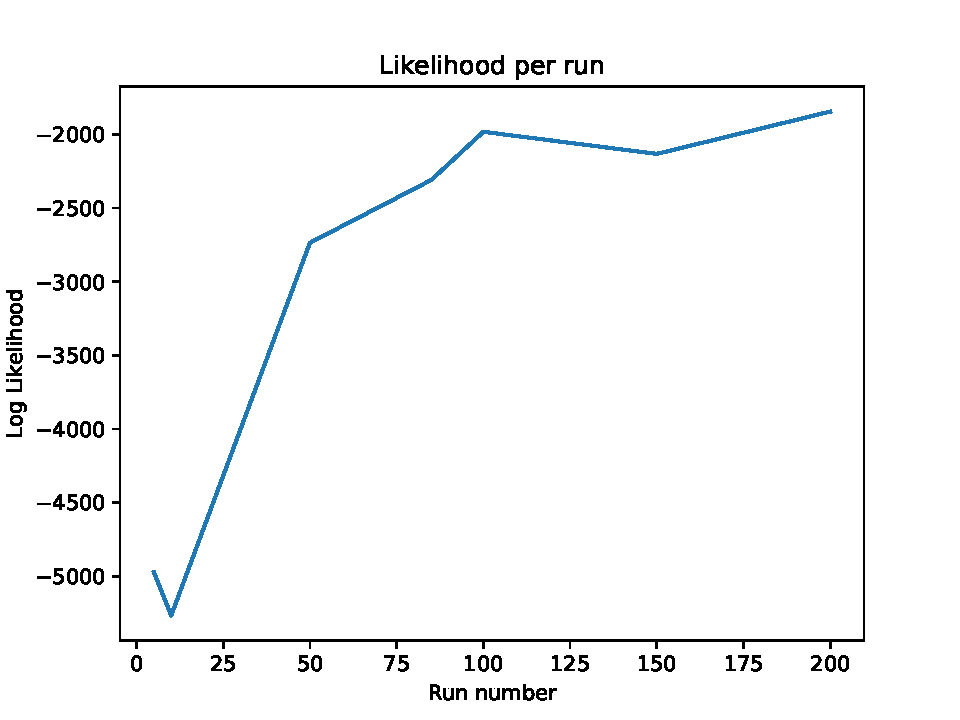
\includegraphics[width=0.8 \textwidth]{3225_lh.pdf}
  \caption{Grafico della likelihood con il metodo nella \autoref{chap:pso-adapt-calculate-5}}
  \end{minipage}
  \begin{minipage}{.45 \textwidth}
    \centering
    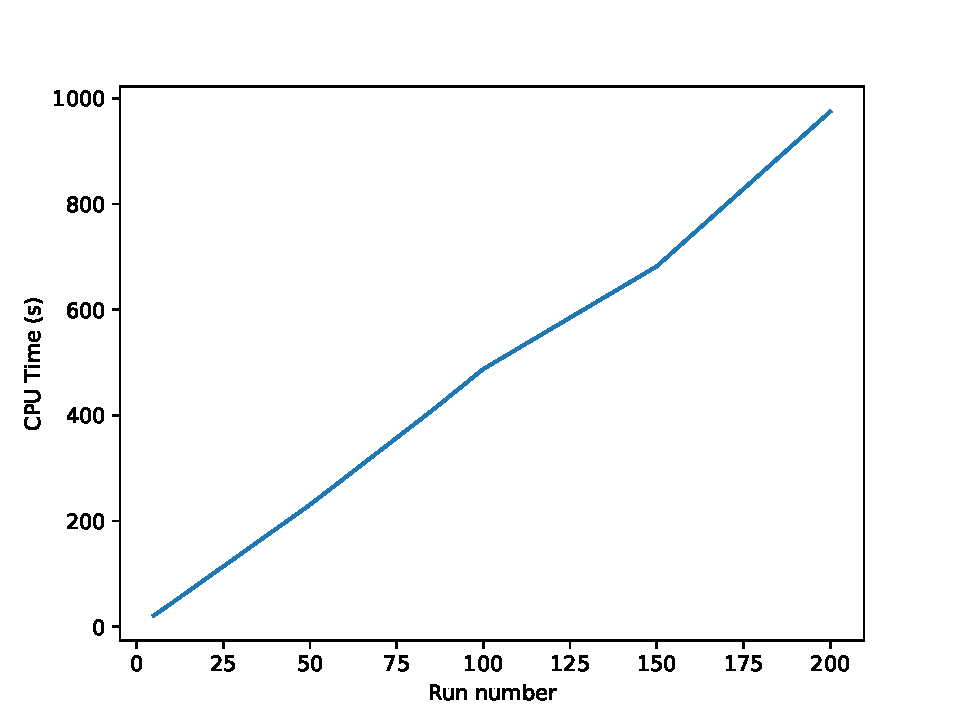
\includegraphics[width=0.8 \textwidth]{3225_cpu.pdf}
    \caption{Grafico del tempo con il metodo nella \autoref{chap:pso-adapt-calculate-5}}
  \end{minipage}
  \label{fig:pso-adapt-calculate-1-graph}
\end{figure}

\begin{figure}[!h]
  \centering
  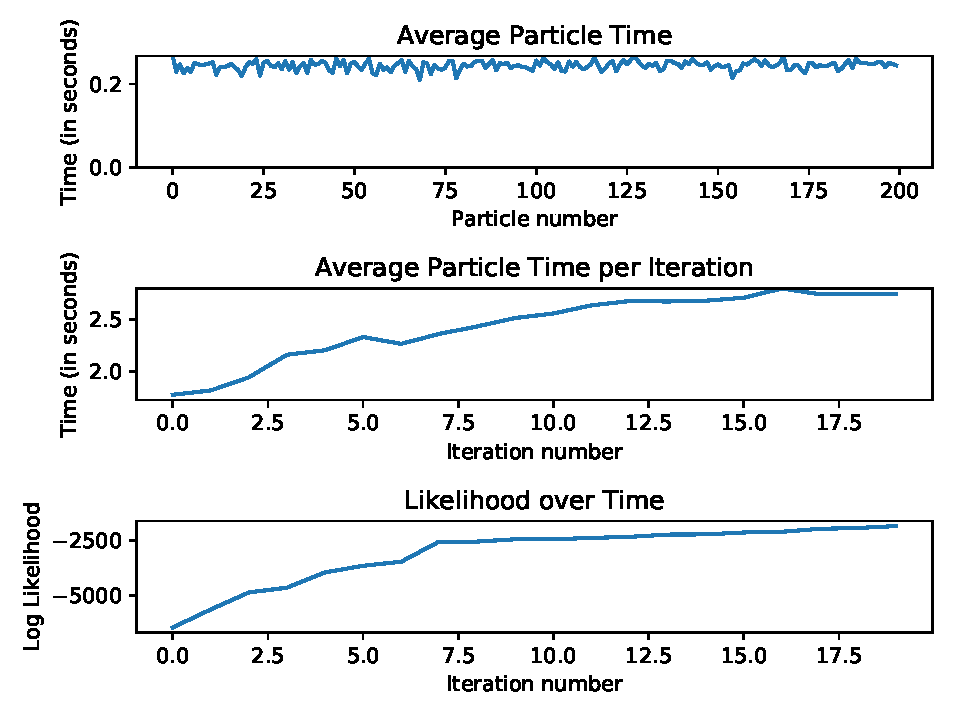
\includegraphics[width=0.8 \textwidth]{3225_data.pdf}
  \caption{Grafici sui tempi ed il miglioramento della likelihood con il passare del tempo con il metodo nella \autoref{chap:pso-adapt-calculate-5}}
  \label{fig:pso-adapt-calculate-4-data}
\end{figure}

\begin{figure}[!h]
  \centering
  \scalebox{0.7}{
  \begin{forest}
    germline
    [{germline} 
    [{3} 
    [{22} 
    [{25} 
    [{18} 
    [{4} 
    [{11} 
    [{9} 
    [{13} 
    [{29} 
    [{1} 
    [{20} 
    [{21} 
    [{6} ]
    [{30} 
    [{17} 
    [{19} 
    [{28} 
    [{12} 
    [{27} 
    [{10} 
    [{7} 
    [{8} 
    [{16} 
    [{15} ]]]]]]]]]]
    [{23} ]
    [{24} 
    [{14} ]
    [{2} ]]]
    [{5} 
    [{26} ]]]]]]]]]]]]]]]
  \end{forest}
  }
  \caption{Albero inferito con il metodo nella \autoref{chap:pso-adapt-calculate-5}}
  \label{fig:pso-adapt-calculate-5-tree}
\end{figure}

\section{Considerazioni aggiuntive}
\label{chap:pso-extra}
Al fine di poter eseguire delle analisi e considerazioni sui risultati ottenuti sono stati fatti diversi accorgimenti sul progetto, di seguito analizzati.

\subsection{Riproducibilità}
\label{chap:pso-extra-ripro}
Durante lo sviluppo di un software può capitare di dover rappresentare una situazione, come un bug, una feature, o un risultato particolare. Questa necessità dà luogo al problema della \textit{riproducibilità}, che implica la possibilità allo sviluppatore o a terzi di poter eseguire il software con parametri comuni al fine di ottenere gli stessi risultati e situazioni. Questo obiettivo è stato raggiunto con diversi accorgimenti, come l'elevata flessibilità di configurazione da linea di comando (descritta in dettaglio nel \autoref{chap:pso-extra-guide}) e la possibilità di poter manipolare gli eventi aleatori fissando un \textit{seed}\footnote{Un numero, o vettore, utilizzato per inizializzare un generatore pseudo-casuale di numeri, come quello utilizzato dalla libreria \textit{random} di Python}.

\subsection{Guida allo strumento nello stato attuale}
\label{chap:pso-extra-guide}

\subsection{Parallelizzazione}
\label{chap:pso-extra-paral}
Tutti i test effettuati in questa sezione sono stati effettuati seguendo l'algoritmo del PSO, cioè in maniera iterativa. È stato possibile implementare un sistema di parallelizzazione dei processi. Ogni processo può eseguire un'iterazione di una particella per volta, riducendo drasticamente i tempi di esecuzione.
Non viene però utilizzata la tecnica di parallelizzazione durante i test, poiché questa aggiunge un fattore di aleicità collegato alla terminazione anticipata dei processi.